\renewcommand{\chaptername}{Cap\'itulo}
\chapter{Planteamiento del problema}
\label{Planteamiento}

\section{Introducci\'on}

El acceso abierto (en adelante AA) es digital, en l\'inea, libre de cargo y libre de la ma\-yo\-r\'ia de restricciones de derechos de autor y licencias; elimina las barreras de precios por suscripciones, cuotas o pago de licencias \cite{PeterSuber2015}. Existen diversos tratados y convenciones internacionales que promueven el AA del p\'ublico en general a la literatura cient\'ifica y acad\'emica de manera digital representada en revistas, tesis, art\'iculos, memorias de eventos, libros, entre otros recursos digitales. En ingl\'es, las siglas para el AA son \textit{OA} de \textit{Open Access}.\newline

La propuesta del AA se plante\'o en la Iniciativa de Budapest en 2002, durante un evento organizado por el Instituto de la Sociedad Abierta (\textit{Open Society Institute}); en 2003, se llev\'o a cabo la Declaraci\'on de Berl\'in sobre el AA al conocimiento en las ciencias y las humanidades \cite{para2010abierto}.
Para \cite{BeneficiosAA}, el AA ofrece a las Instituciones de Edu\-caci\'on Superior (IES) y Centros de Investigaci\'on (CIs) beneficios como los siguientes: 
\begin{itemize}
\item Rendici\'on de cuentas transparente ante la sociedad con respecto a la inversi\'on p\'ublica
\item Incremento en la difusi\'on e impacto de la producci\'on cient\'ifica  
\item Fomento de la producci\'on cient\'ifica y acad\'emica, aumenta las posibilidades de acceso 
\item Facilita el intercambio de informaci\'on entre IES, CIs, comunidades locales, nacionales e internacionales
\item Garantiza la preservaci\'on electr\'onica de recursos documentales digitales
\end{itemize}
 
Entre los beneficiarios del AA est\'an los autores, las comunidades cient\'ificas, acad\'emicas y usuarios de \emph{repositorios institucionales} (RIs). Los RIs son plataformas tecnol\'ogicas dise\~{n}adas para almacenar, preservar y difundir documentos digitales que se distribuyen bajo los t\'erminos de las pol\'iticas de AA, son un medio de divulgaci\'on (\textit{ruta verde}) o de publicaci\'on (\textit{ruta dorada}), de los contenidos producidos por una instituci\'on o comunidad \cite{RutaVerdeDorada}. \newline

Seg\'un \cite{EcosistemasdelAA}, un repositorio institucional (RI) es un conjunto de servicios prestados por las universidades y organismos de investigaci\'on a la   comunidad para recopilar, ad\-mi\-nis\-trar, difundir, y preservar la producci\'on documental digital, cualquiera que sea su tipolog\'ia, a trav\'es de la creaci\'on de una colecci\'on digital organizada, abierta e interoperable que emplea el protocolo OAI-PMH, con el fin de garantizar un aumento en la visibilidad e impacto de la propia instituci\'on. \newline

En Diciembre de 2018, seg\'un el sitio OpenDOAR \cite{OpenDOAR}, directorio de repositorios de AA de la Universidad Nottingham, exist\'ian 3,779 repositorios alrededor del mundo, de los cuales (46\%) se encuentran en Europa, el 27\% en Norteam\'erica y s\'olo el 0.9\% en M\'exico. En M\'exico, al 9 de Noviembre del 2019, la p\'agina web del Repositorio Nacional (RN) \cite{RepositorioNacional} reporta la existencia de 105 repositorios de Ciencia Abierta (CA) e INDEXE, Sistema de B\'usqueda de la Red Mexicana de Repositorios Institucionales (REMERI) \cite{RI_REMERI} indica 100 RIs comprometidos con la divulgaci\'on de sus contenidos institucionales y tem\'aticos. De acuerdo con datos de la red REMERI, 
m\'as del 45\% de RIs pertenecen a instituciones p\'ublicas, siendo la Universidad Nacional Aut\'onoma de M\'exico (UNAM), la instituci\'on con mayor n\'umero de repositorios y documentos publicados \cite{RI_REMERI}. \newline

Seg\'un datos de OpenDOAR \cite{OpenDOAR}, la distribuci\'on del \textit{software} empleado para la implementaci\'on de los 3.779 RIs es como sigue:  \textit{DSpace} \cite{DSpaceRef} (44.2\%), \textit{EPrints} (13.4\%), \textit{Digital Commons} (4.7\%) y \textit{WEKO} (2.7\%). A diferencia de \textit{Digital Commons} que es un \textit{software} licenciado por la empresa \textit{Bepress}, \textit{WEKO}, \textit{EPrints} y \textit{DSpace} cuentan con licencia libre, por lo que su uso se ha extendido en m\'ultiples IES, CIs y otras organizaciones.\newline

Por un lado, \textit{EPrints} \cite{EPrints} se desarroll\'o de la Universidad de Southampton en el Reino Unido del 2010, esta plataforma soporta la preservaci\'on, diseminaci\'on y generaci\'on de reportes para instituciones que requieran que servicios de AA, tambi\'en permite la cons\-truc\-ci\'on de repositorios de educaci\'on abierta (en ingl\'es, \textit{open education}) y bancos de datos para investigaci\'on (\textit{research data}). EPrints se emplea como medio de integraci\'on con redes sociales. Por otro lado, \textit{DSpace} \cite{DSpaceRef} surgi\'o como proyecto desarrollado en sus inicios por el Instituto Tecnol\'ogico de Massachusetts (MIT) en el a\~{n}o 2002 en conjunto con los Laboratorios HP. Actualmente, se mantiene en la fundaci\'on \textit{DuraSpace} que entre sus objetivos se encuentran la innovaci\'on en tecnolog\'ias de AA y basadas en nube, principalmente para bibliotecas, universidades, CIs y organizaciones de patrimonio cultural. DSpace soporta el almacenamiento de tesis, administraci\'on de registros electr\'onicos, preservaci\'on digital y publicaci\'on. Los RIs que interoperan con el RN \cite{RepositorioNacional} emplean en su mayor\'ia (m\'as del 90\%) una versi\'on de DSpace.  Una comparaci\'on que considera aspectos de funcionalidad, elementos t\'ecnicos y de administraci\'on entre las plataformas EPrints y DSpace se presenta en \cite{EvaluacionDeUsabilidad}.\newline

En EPprints y DSpace la interoperabilidad por omisi\'on se implementa al utilizar el Protocolo de la Iniciativa de Archivos Abiertos para la Diseminaci\'on de metadatos OAI-PMH\footnote{OAI-PMH corresponde a las siglas de \textit{Open Archives Initiative Protocol for Metadata Harvesting}} \cite{Lagoze2005} y el est\'andar de metadatos Dublin Core \cite{DublinCore}. En el RI de la Universidad Polit\'ecnica de Puebla, en adelante RI-UPPue, est\'a soportado en la versi\'on 5.2 de DSpace. En esta tesis se identifica como problem\'atica para la comunidad universitaria lo siguiente:

\begin{itemize}
\item Los mecanismos de recuperaci\'on de informaci\'on disponibles desde la interfaz del RI-UPPue s\'olo distinguen entre el autor principal y los coautores de los documentos; a la fecha, no se puede determinar un rol de los coautores como asesor o sinodal si se trata de una tesis, o autor principal, segundo o tercer autor si se trata de un art\'iculo

\item  Existe \textit{ambig\"{u}edad} en la interpretaci\'on de los datos descriptivos o \emph{metadatos} cuando se depositan documentos en el RI-UPPue, por ejemplo, qu\'e se debe colocar dentro del elemento \emph{contributor} al depositar una tesis de maestr\'ia

\item A pesar de que otras IES que interoperan con el RN tal como el RI-UPPue y de que emplean la plataforma DSpace, la interpretaci\'on de los datos exportados est\'a sujeta a los usuarios finales, dado que \'esta se realiza por omisi\'on \'unicamente en el formato CSV\footnote{CSV corresponde a las siglas de \emph{Comma Separated Values}}.

\end{itemize}

Previamente, en la UPPue se desarroll\'o un modelo sem\'antico u ontolog\'ia denominada  \emph{Onto4AIR}, es un producto de software que representa formalmente conocimiento de dominio y operativo de los RIs, hace \'enfasis en los documentos, los tipos de usuario y sus relaciones \cite{representacionSemantica}. La tesis propone utilizar instancias de esta ontolog\'ia y tecnolog\'ias sem\'anticas como alternativas para atender la problem\'atica anterior, de manera que los objetivos son: 

\section{Objetivo general} 
Extender los mecanismos de b\'usqueda de tesis, art\'iculos y carteles del RI-UPPue utilizando tecnolog\'ias sem\'anticas para atender necesidades de informaci\'on de usuarios del RI-UPPue

\subsection{Objetivos espec\'ificos}

\begin{itemize}

     \item Describir la funcionalidad del componente RDF de la plataforma DSpace 6.2 
     
     \item  Integrar datos de tesis de maestr\'ia, art\'iculos y carteles del RI-UPPue a instancias de la ontolog\'ia Onto4AIR validando su consistencia l\'ogica de forma autom\'atica mediante razonadores
     
     \item Dise\~{n}ar e implementar un servicio web tipo REST que permita recuperar datos de dos RIs utilizando instancias de la ontolog\'ia Onto4AIR
    
   \end{itemize}
   
%% La Figura \ref{actividades_objetivos} muestra algunas de las tareas requeridas para alcanzar los objetivos. 
%% Esta figura se pasara al cap. 3

%%\begin{figure}[!ht]
%%    \centering
%%    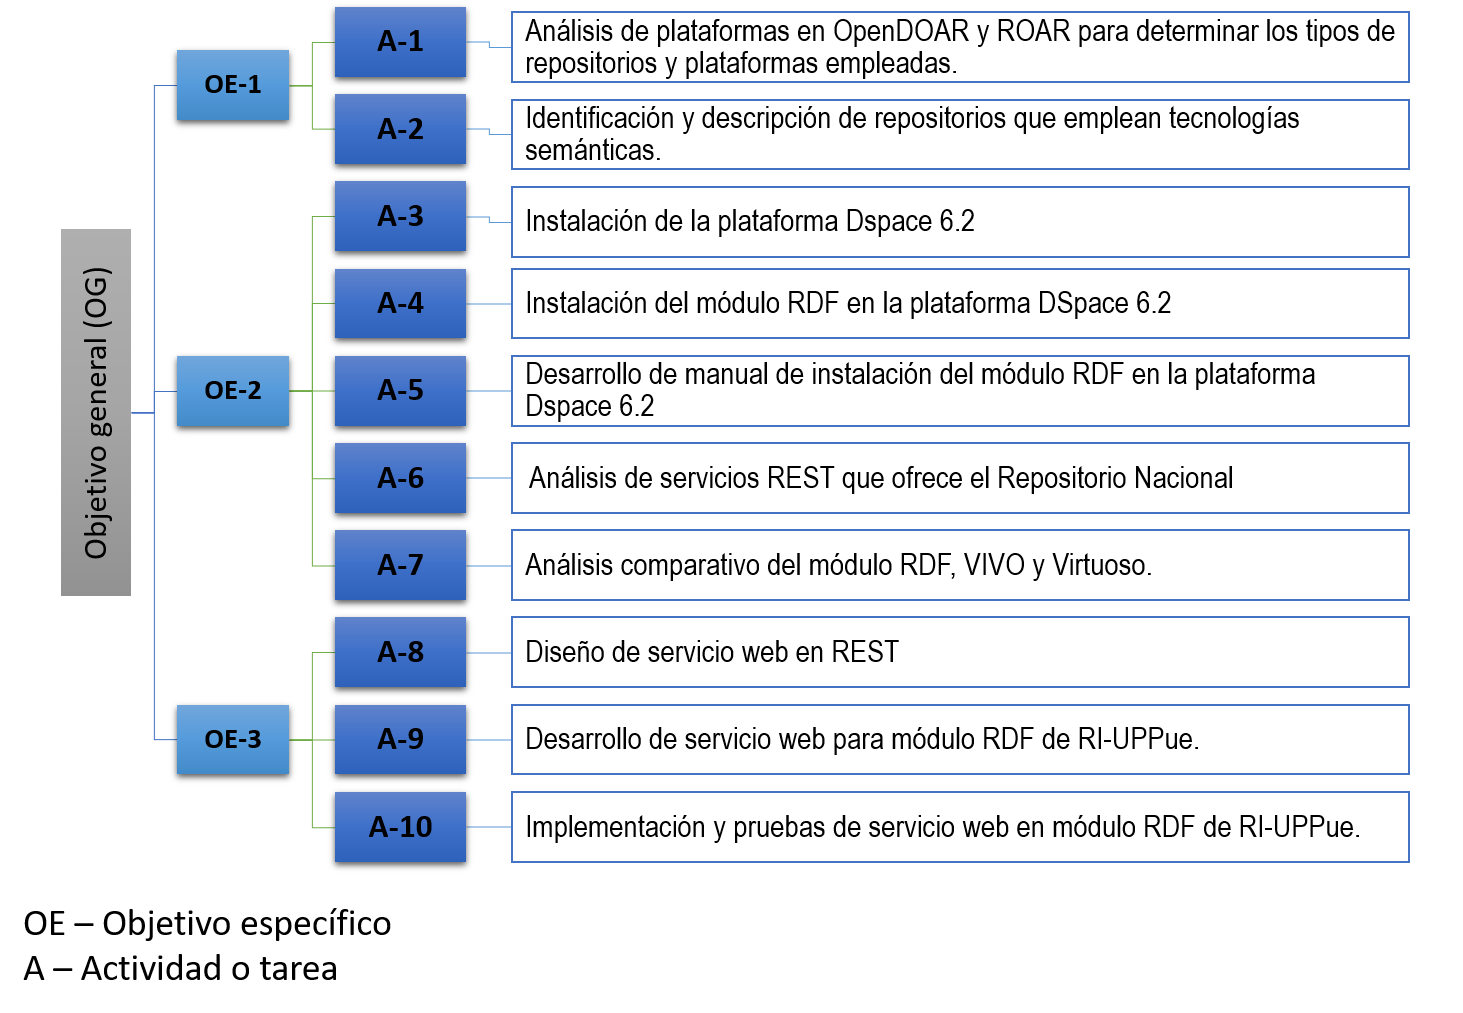
\includegraphics[width=12cm]{figures/Actividades_Dic_2018.png} %NOMBRE DE LA FIGURA y TAMANIO
%%    \caption{Tareas a desempe\~{n}ar para el desarrollo del servicio web} %PIE DE LA IMAGEN
%%    \label{actividades_objetivos}
%%\end{figure}

\section{Justificaci\'on}

En los \'ultimos a\~{n}os, diferentes IES, CIs y comunidades se han sumado el esfuerzo de promover el AA a sus contenidos cient\'ificos mediante RIs que en su mayor\'ia emplea modelos de datos relacionales para almacenar informaci\'on. De acuerdo con \cite{ASWebQuest}  y \cite{GuideCreatingOntology}, el uso de tecnolog\'ias sem\'anticas como las ontolog\'ias se caracteriza por lo siguiente: 

\begin{itemize}
\item Intercambio de datos entre aplicaciones, programas y/o plataformas mediante el lenguaje XML\footnote{XML son las siglas de \textit{eXtensible Markup Language}}  o lenguajes derivados de \'este
\item Las ontolog\'ias permiten gestionar datos incompletos y reutilizar el conocimiento 
\item Los datos en las ontolog\'ias forman conjuntos de datos que son procesables por computadora

\end{itemize}

Los beneficios esperados del desarrollo de la tesis son:
	
	\begin{itemize}
	 \item Recopilaci\'on y divulgaci\'on de datos de producci\'on cient\'ifica y acad\'emica del RI-UPPue en formatos de la web sem\'antica    
         \item Uso de la ontolog\'ia Onto4AIR como alternativa de integraci\'on de informaci\'on sem\'antica a datos provenientes de otros RIs
         \item Extensi\'on de los mecanismos de b\'usqueda y recuperaci\'on del RI-UPPue, recuperaci\'on desde un punto de vista conceptual y no s\'olo textual 
         \end{itemize}

